\section{Classification \& Logistic Regression}
\subsection{Binary Classification}
\begin{itemize}
    \item Decision with 2 possible outcomes
    \item Hail in Lausanne (yes/no)
    \item Master admission (admission / no admission)
    \item Based on different data / entity
\end{itemize}

\subsubsection{Decision using Linear Regression}
\begin{itemize}
    \item Train the model with gradient descent
    \item \textbf{Bad Idea!}
    \begin{itemize}
        \item The cost function minimizes the MSE difference in the values of $\hat{y}$ and $y$ and has nothing to do with the classification probabilities!
    \end{itemize}
    \item Models the response (y) and post process the response to compute the probability
\end{itemize}

\subsubsection{The sigmoid function}
\begin{center}
    $sigmoid(y) = \frac{1}{1 + e^{-y}}$
\end{center}
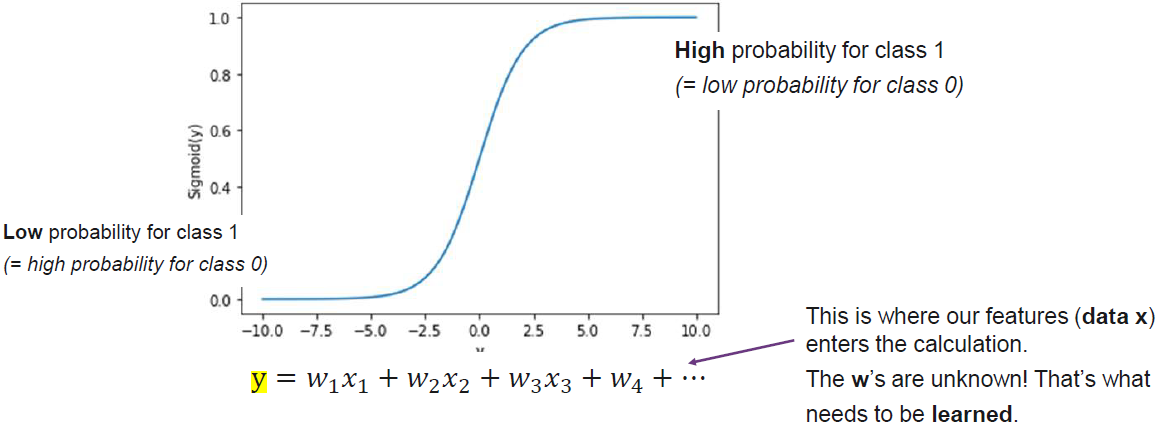
\includegraphics[width=\linewidth]{./img/sigmoid.png}

\textbf{Probabilities}\\
\begin{minipage}{0.59\linewidth}
\begin{itemize}
    \item We can write the estimated probability
    \item For a prediction we can write
\end{itemize}
\end{minipage}
\begin{minipage}{0.4\linewidth}
\begin{center}
    $P(x) = \frac{1}{1 + e^{-(W^{T}x)}}$
\end{center}
\end{minipage}

\textbf{Beispiel:}\\
How likely is it, that a student fit features $x_1=4.5$ and $x_2=5.5$ get accepted and get rejected?\\
\begin{center}
Parameters: $w_1=1, w_2=-0.7, w3=-0.7$\\
\end{center}
\begin{align*}
%$Features: x_1=4.5, x_2=5.5$\\
Pr(accept|x;w) &= \frac{1}{1 + e^{-(w_1*x_1+w_2*x_2+w_3)}} &= 0.49\\
Pr(reject|x;w) &= 1 - Pr(pass|x;w) &= 0.51
%($w_3$ ist wie ein 'Intercept')
\end{align*}

\subsubsection{Maximum Likelihood}
\begin{itemize}
    \item Given all the data points (X,Y) we want to maximize the probability that all the predictions are correct.
    \item For each of the training data, we want to maximize the likelihood of correct prediction
    \item We can use Gradient Descent to find W
\end{itemize}

\subsubsection{Maximum Likelihood Estimation (MLE)}
\textbf{Problem of Probability Density Estimation}
\begin{itemize}
    \item Density estimation is the problem of estimating the probability distribution for a sample of observations from a problem domain
    \item Common Solution $\rightarrow$ Maximum Likelihood Estimation (MLE)
\end{itemize}
\textbf{Maximum Likelihood Estimation (MLE)}
\begin{itemize}
    \item MLE involves defining a likelihood function for calculating the conditional probability of observing the data sample given a probability distribution and distribution parameters
    \item \textit{Goal}: find the optimal way to fit a distribution to the data
    \item MLE versucht den optimalen Wert für den Mittelwert oder die Standardabweichung einer Verteilung zu finden, wenn eine Reihe von Messwerten vorliegen
\end{itemize}
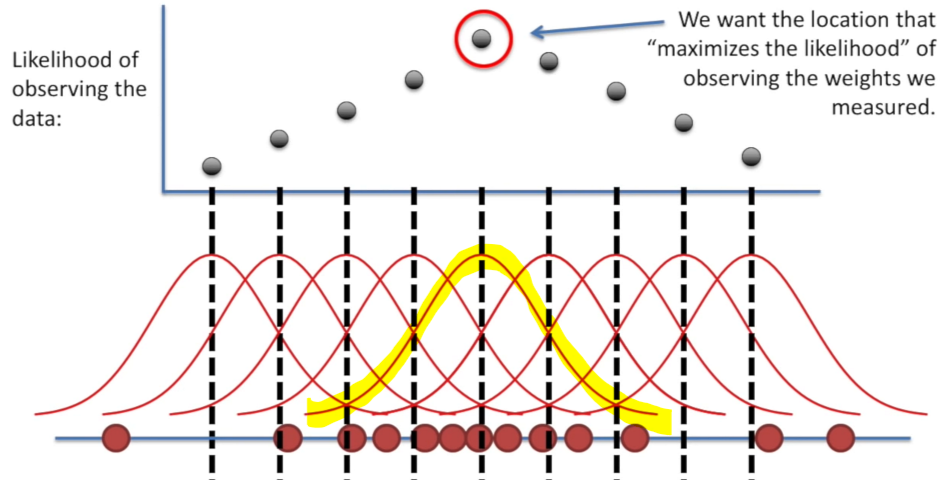
\includegraphics[width=\linewidth]{./img/mle.png}

\subsubsection{Loss Function used in logistic regression}
\begin{center}
    $\frac{-1}{N}\displaystyle\sum_{i = 1}^{N} y_i \ln(p_i) + (1 - y_i) \ln(1 - p_i)$
\end{center}

\subsection{Logistic Regression}
\begin{itemize}
    \item Die (binär) logistische Regressionsanalyse wird angewandt, wenn geprüft werden soll, ob ein Zusammenhang zwischen einer abhängigen binären Variablen und einer oder mehreren unabhängigen Variablen besteht.
    \item Mit binärerer logistic Regression können die Wahrscheinlichkeiten für das Eintreffen von Ereignissen vorausgesagt werden.
    \item Logistic Regression predicts whether something is \textbf{True} or \textbf{False}, instead of predicting something continuous like size (Linear Regression)
    \item Logistic Regression doesn't have the same concept of a "residual", so it can't use least squares and it can't calculate $R^2$
    \begin{itemize}
        \item Instead, it uses \textbf{mamimum likelihood}
    \end{itemize}
    \item \textit{Beispiel}:  Ausgang einer Aufnahmeprüfung $\rightarrow$ (Angenommen oder Abgelehnt = binäre logistic Regression (2 Möglichkeiten))
    \begin{itemize}
        \item Y-Achse: Wahrscheinlichkeit (1=sicher angenommen, 0=sicher abgelehnt)
        \item X-Achse: Intelligenz (je Intelligenter desto höher die Chance, angenommen zu werden)
        \item Je steiler die Kurve, desto besser die Vorhersage (des Prediktors)
    \end{itemize}
\end{itemize}

\begin{center}
    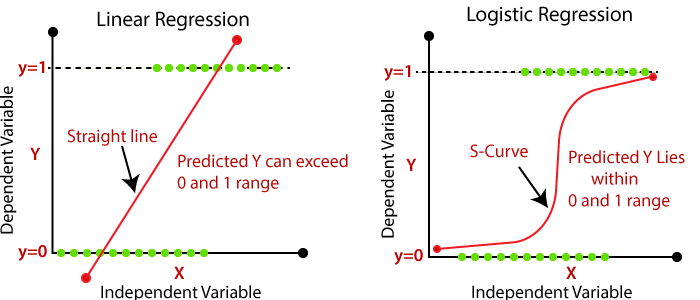
\includegraphics[width=0.8\linewidth]{./img/logistic_regression.png}
\end{center}
